\documentclass[a4paper]{article}

\usepackage[]{amsmath} 
\usepackage[]{amsthm} 
\usepackage[]{amssymb} 

\usepackage[backend=biber, style=alphabetic]{biblatex} 
\addbibresource{../bib/mat2000.bib}
\usepackage[]{url} 
\urlstyle{sf}

\usepackage[]{graphicx} 
\usepackage[]{wrapfig} 
\usepackage[]{caption} 
\usepackage[]{subcaption} 

\usepackage[]{enumerate} 

\usepackage[]{cleveref} 

\theoremstyle{definition}
\newtheorem{defn}{Definition}
\newtheorem{exmpl}{Example}

\theoremstyle{plain}
\newtheorem{lma}{Lemma}
\newtheorem{crl}{Corollary}

\newcommand{\C}{\ensuremath{\mathbb{C}}}
\newcommand{\proj}{\ensuremath{\mathbb{P}}}
\renewcommand{\hom}{\ensuremath{h_{\mathrm{hom}}}}

\title{Visualizing Algebraic Surfaces}
\author{Ivar Haugal{\o}kken Stangeby}
\date{\today}

\begin{document}

    \begin{titlepage}
    \maketitle

    \begin{figure}[htb]
        \centering
        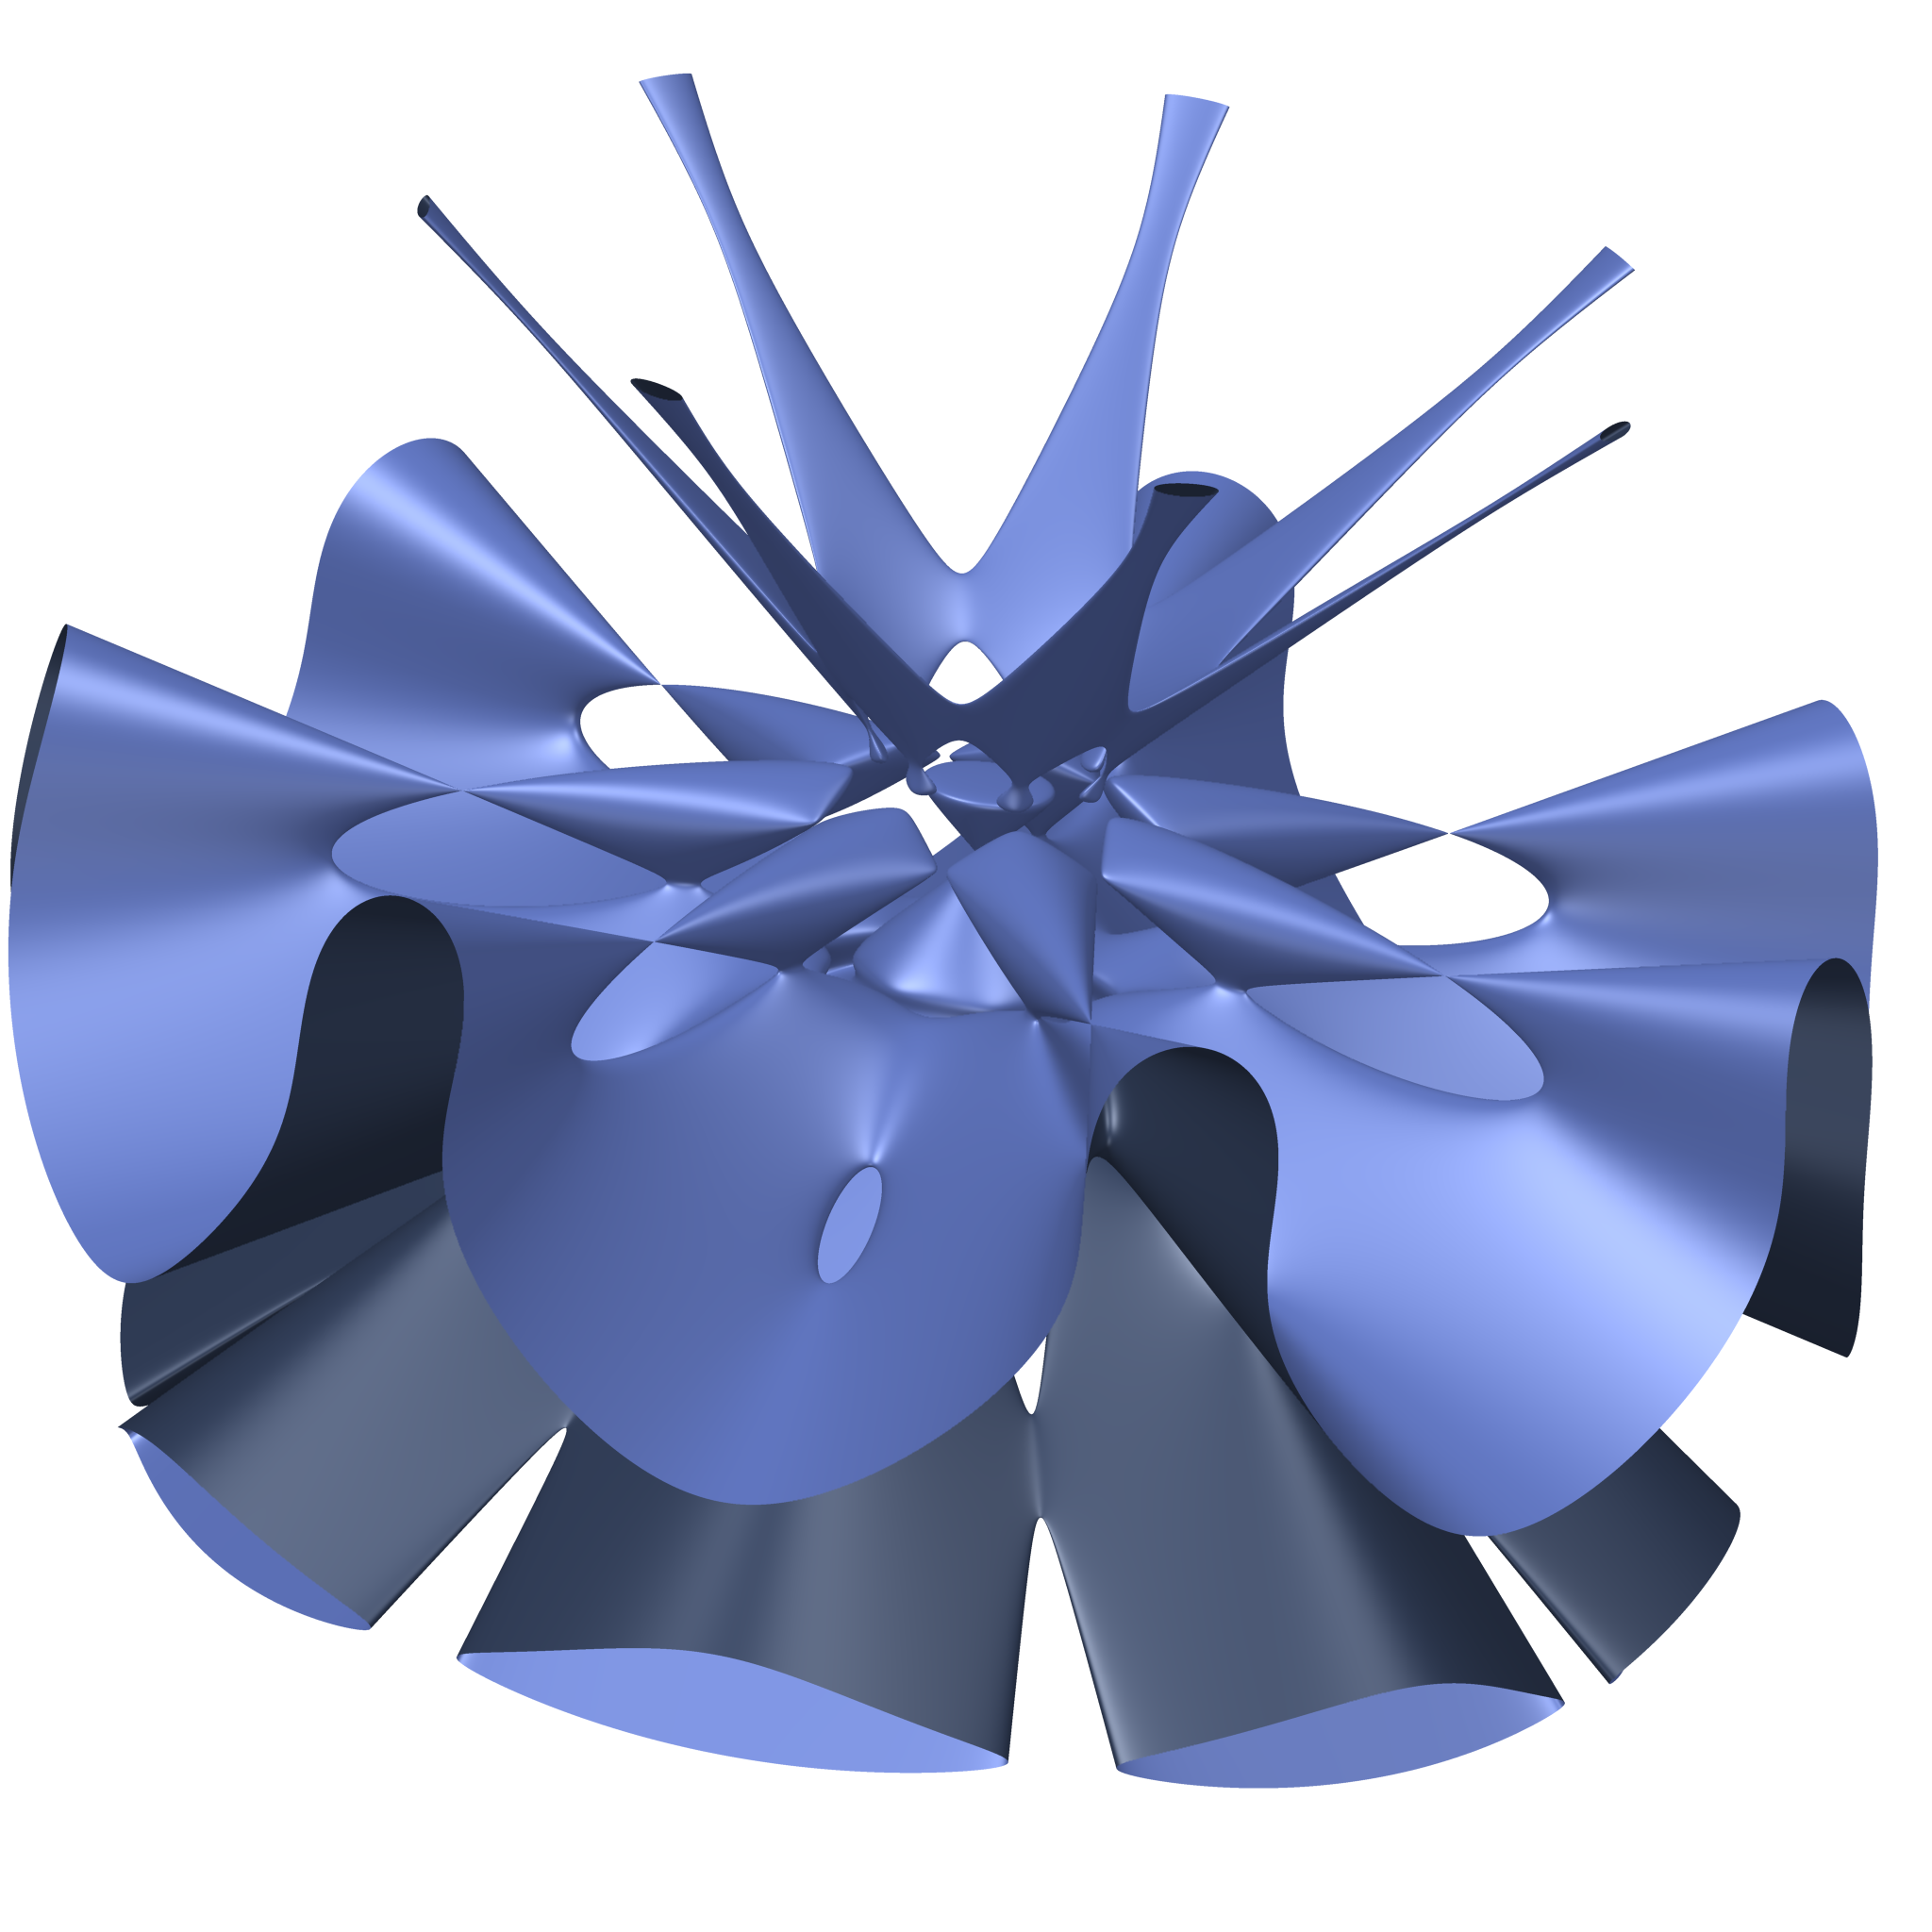
\includegraphics[width=0.8\linewidth]{../pictures/labs_septic.png}
    \end{figure}
    \end{titlepage}
    \tableofcontents

    \section{An Informal Introduction}
    \label{sec:an_informal_introduction}
    
    In this section we briefly look at the natural construction of the
    mathematical objects we are interested in studying in the rest of this
    paper.

    \subsection{Real Algebraic Curves}
    \label{sub:real_algebraic_curves}
    
    From elementary mathematics one learns about real valued functions, $f(x)$,
    and how to graph these functions by setting $y = f(x)$ and plotting points
    in the $(x, y)$-plane. Now, the \emph{graph of a function} is something of
    a peculiarity, because it comes with some restrictions. Not all curves in
    the $(x, y)$-plane correspond to functions. The method for verifying
    whether a certain ''graph'' corresponds to a function or not typically
    taught in school is the \emph{vertical line test}. 

    Having an equation $y = f(x)$ we can form what we call the \emph{equation
    of a curve at zero}. We define a new function in two variables
    \begin{equation}
        \label{eq:equation_at_zero}
        g(x, y) = y - f(x) = 0.
    \end{equation}
    If the function $f(x)$ is a polynomial in the variable $x$ with certain
    coefficients we call the function graph of $f(x)$ \emph{algebraic}.

    Generally speaking, we call a curve defined by \cref{eq:equation_at_zero}
    an \emph{algebraic curve} if the function $g(x, y)$ is a polynomial in two
    variables, $x$ and $y$. Mathematically, this can be expressed as
    \begin{equation}
        \label{eq:algebraic_curve}
        g(x, y) = \sum^{}_{i, j} a_{i_j}x^{i}y^{i}.
    \end{equation}
    
    However, if this distinction between a graph and a curve is to be justified
    there has to be some curves that are not graphs. One of the first examples
    one encounter of a curve not corresponding to a function is what you get
    when you set $y^2 = x^3$. This curve does not pass the vertical-line-test
    and is therefore something different from a graph. Similarly, the equation
    $y^2 = x^3 - x^2$ defines a curve that again is not a graph. These are
    shown in \cref{fig:curves_not_graphs}. These curves exhibit \emph{singular
    points} at $(0, 0)$. 
    
    \begin{figure}[h]
        \centering
        \begin{subfigure}{0.5\textwidth}
            \centering
            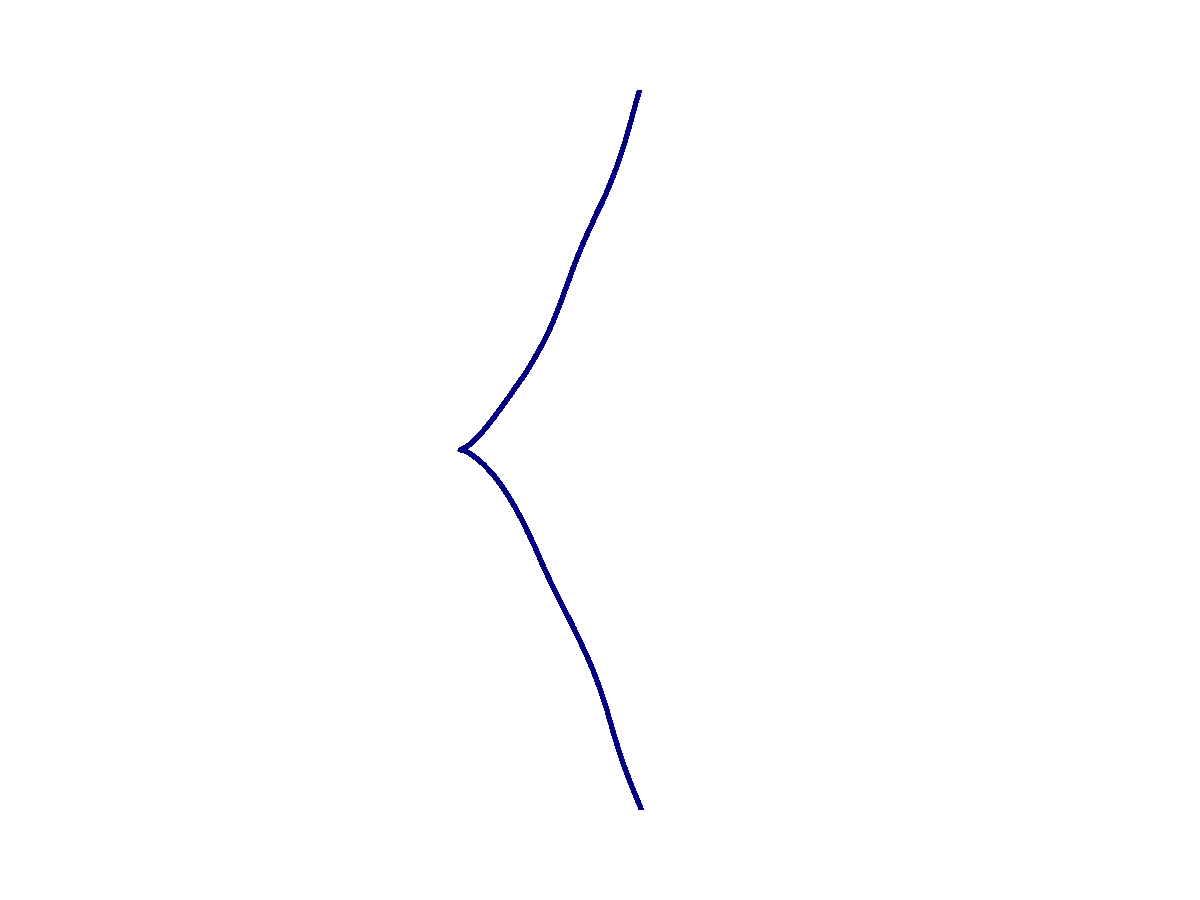
\includegraphics[width=1.0\linewidth]{../pictures/cusp.pdf}
            \caption{$g(x, y) = y^2 - x^3 = 0$}
        \end{subfigure}%
        \begin{subfigure}{0.5\textwidth}
            \centering
            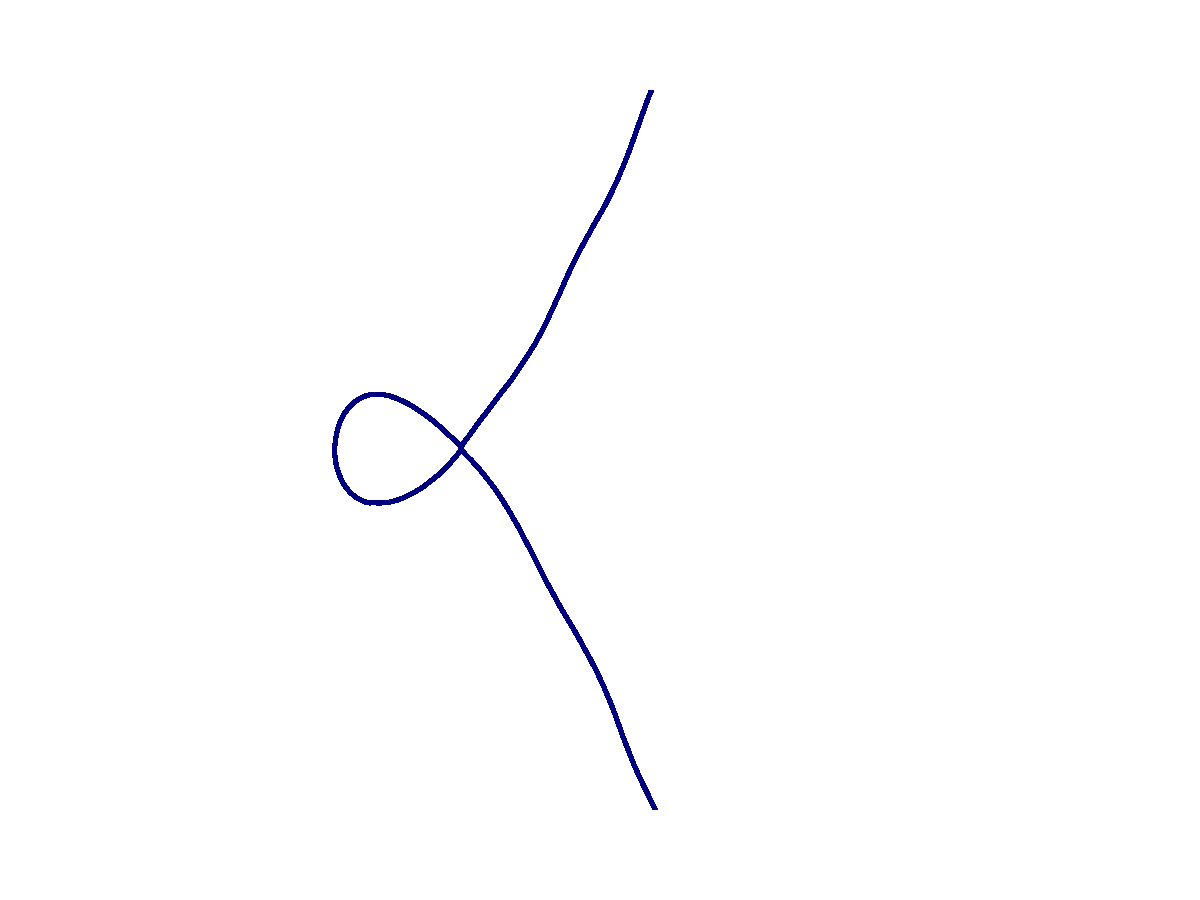
\includegraphics[width=1.0\linewidth]{../pictures/double_point.pdf}
            \caption{$g(x, y) = y^2 - x^3 + x^2 = 0$}
        \end{subfigure} 
        \caption{Examples of curves that are \emph{not} graphs given by their
        functions $g(x, y)$}.}
        \label{fig:curves_not_graphs}
    \end{figure}
    
    With what we have so far, we can move up a dimension. Instead of
    considering curves in the $(x, y)$-plane we can look at surfaces in the
    $(x, y, z)$-space. We, as we did with $g(x, y)$ above, define a function
    $h(x, y, z) = z - g(x, y)$. The surfaces are given by equations on the form
    $h(x, y, z) = 0$. These surfaces are called algebraic if $h(x, y, z)$ is a
    polynomial in the variables $x, y, z$. Again, mathematically, this is
    expressed as
    \begin{equation}
        \label{eq:algebraic_surfaces}
        h(x, y, z) = \sum^{}_{i, j, k} a_{ijk}x^iy^jz^k.
    \end{equation}

    \subsection{Going Complex}
    \label{sub:going_complex}

    The surfaces considered so far are over the real numbers, i.e, the
    coefficients $a_{ijk}$ are real numbers. We can instead work over the
    complex numbers where the surfaces are given by an equivalent equation, but
    where the coefficients now are complex numbers\footnote{We will come back
    to why we make this transition when we talk about sets being algebraically
    closed or not.}:
    \begin{equation}
        \left\{ (x, y, z) \in \C \mid h(x, y, z) = 0 \right\}.
    \end{equation}
    Again, doing the same trick (one-trick ponies) we can now define $w = h(x,
    y, z)$ and look at the equations $w - h(x, y, z) = 0$ in the $(x, y, z,
    w)$-space. Now, we are stuck with an equation in four variables. With only
    three degrees of freedom to work with when visualizing these objects we
    encounter an obstacle. How do we know what these surfaces look like? This
    brings us to the world of \emph{projective geometry}.

    \section{Projective Geometry}
    \label{sec:projective_geometry}
    
    The way we work these surfaces in four variables is by introducing a new
    variable making the polynomial terms all have the same degree.  This is
    called \emph{homogenizing} the polynomial $h(x, y, z)$. We first want to
    introduce some definitions.

    Quite informally, projective space formalizes the notion of parallell lines
    intersecting at infinity. In order to get a better understanding of the
    general projective space $\proj^n$ we will first construct the
    \emph{projective plane} $\proj^2(\C)$.

    \subsection{The Projective Plane}
    \label{sub:the_projective_plane}
    
    According to \cite{Wik16} there are three equivalent definitions:
    \begin{enumerate}
        \item The set of all lines in $\C^3$ passing through the origin $(0, 0,
            0)$. Every such line meets the \emph{sphere} of radius one centered
            in the origin exactly twice, say in $P = (x, y, z)$ and its
            antipodal point $(-x, -y, -z)$.

        \item\label{item:sphere} The points on the sphere $S^2$, where every point $P$ and its
            antipodal points are not distinguished. For example, the point $(1,
            0, 0)$ is identified with the point $(-1, 0, 0)$.

        \item The set of equivalence classes of $\C^3 \setminus \left\{ 0
            \right\}$ where two points $P$ and $P'$ are considered equivalent
            if and only if there is a non-zero $\lambda \in \C$ such that $P =
            \lambda P'$.
    \end{enumerate}

    The last definition is the one seemingly most used, and is therefore the
    one we will employ here. Note that the elements in the projective plane are
    equivalence classes of points in $\C^3$. We denote an element in
    $\proj^2(\C)$ as $\left[ x : y : z \right]$. These elements are commonly
    referred to as \emph{homogenous coordinates}. We state this formally in a
    definition.

    \begin{defn}[The projective plane]
        Let $\sim$ be the equivalence relation on $\C^3$ defined by
        \begin{equation}
            \notag
            (x, y, z) \sim (x', y', z') \iff (x', y', z') = \lambda(x, y, z),
        \end{equation}
        where $\lambda$ is some non-zero scalar in $\C$. We denote the
        equivalence class of $(x, y, z)$ as $\left[ x : y : z \right]$ and we
        define the \emph{projective plane} as the set
        \begin{equation}
            \notag
            \proj^2(\C) = \left\{ \left[ x : y : z \right] \mid (x, y, z) \in
            \C^3 \setminus \left\{ 0 \right\}\right\}.
        \end{equation}
    \end{defn}

    We can now look at an interesting subset of $\proj^2(\C)$, namely the set
    of points $\left[x : y : z \right]$ where $z \neq 0$. Remembering the
    identification from the above definition, these are equivalent to $\left[
    \frac{x}{z} : \frac{y}{z} : 1 \right]$ where $\lambda = 1 / z$. If we
    consider definition \cref{item:sphere} from above, this corresponds to the
    set of points on the northern hemisphere of $S^2$ not including the circle
    of intersection in the $(x, y)$-plane. Similarly, we can look at the set of
    points $\left[ x : y : 0 \right]$. This correponds, in $S^2$, to the circle
    of intersection in the $(x, y)$-plane.

    We can now take the notion of the
    projective plane and generalize this to $n$ dimensions.
    
    \subsection{Projective Space}
    \label{sub:projective_space}
    
    The general definition of projective $n$-space is completely anologous to
    the definition of the projective plane, the set of lines in $\C^{n+1}$
    passing through the origin, however we include a formal definition for
    completeness.

    \begin{defn}[The projective space of dimension $n$]
        Let $\sim$ be an equivalence relation on $\C^{n+1} \setminus \left\{ 0
        \right\}$ defined by
        \begin{equation}
            \notag
            \left( x_1, \ldots, x_{n+1} \right) \sim \left( x_1', \ldots,
            x_{n+1}' \right) \iff \left( x_1', \ldots, x_{n+1}' \right) =
            \lambda \left( x_1, \ldots, x_{n+1} \right)
        \end{equation}
        where $\lambda$ is some non-zero complex number. We then denote the
        equivalence class of $\left( x_1, \ldots, x_{n+1} \right)$ by $\left[
        x_1 : \ldots : x_{n+1} \right]$ and define the \emph{projective space
        of dimension $n$} as the set
        \begin{equation}
            \notag
            \proj^n{\C} = \left\{ \left[ x_1 : \ldots : x_{n+1} \right] \mid
            \left( x_1, \ldots, x_{n+1} \right) \in \C^{n+1} \setminus \left\{
            0 \right\} \right\}.
        \end{equation}
    \end{defn}
    
    \section{Algebraic Surfaces}
    \label{sec:algebraic_surfaces}
    
    We are now equipped with what we need to again look at our algebraic
    surfaces defined by $h(x, y, z) = 0$. The solutions to this equation are
    points in $\C^4$. We homogenize this polynomial by introducing the variable
    $w$ and evaluating $h$ at the points $x \to x/w$, $y \to y/w$ and $z \to
    z/w$ and then multiply by $w^d$ where $d$ is the degree of the polynomial
    $h(x, y, z)$. 

    \begin{defn}[Homogenized polynomial]
        Let $h(x, y, z)$ be a polynomial in $x, y, z$ of degree $d$. 
        The homogenized polynomial $\hom(w, x, y, z)$ is given by
        \begin{equation}
            \notag
            \hom(w, x, y, z) = w^d h \left( \tfrac{x}{w}, \tfrac{y}{w}, \tfrac{z}{w} \right).
        \end{equation}
        It follows that each non-zero term in this polynomial has the same
        degree.
    \end{defn}
    The property that each non-zero term has the same degree in a homogeneous
    polynomial gives rise to a very important property which relates directly
    to the projective geometry introduced above.\footnote{This following
    property can be seen directly by visualizing the homogenous polynomial
    formed by a polynomial $g(x, y)$ and noticing that the figure does not
    change when zooming in or out.}
    
    \begin{crl}
        If $\hom$ is an homogeneous polynomial formed by homogenizing the
        polynomial $h(x, y, z)$ of degree $d$, then
        \begin{equation}
            \notag
            \hom(\lambda w, \lambda x, \lambda y, \lambda z) = \lambda^d \hom(w, x, y, z).
        \end{equation}
    \end{crl}
    \begin{proof}
        We simply compute the left hand side:
        \begin{align*}
            \notag
            \hom(\lambda w, \lambda x, \lambda y, \lambda z) &= (\lambda w)^d h
            \left( \tfrac{\lambda x}{\lambda w}, \tfrac{\lambda x}{\lambda w},
            \tfrac{\lambda x}{\lambda w}\right) \\ &= \lambda^d \hom(w, x, y,
            z).
        \end{align*}
    \end{proof}
    Since we are working with homogenous coordinates, the condition $\hom(w, x,
    y, z) = 0$ is well defined on the equivalence class discussed above,
    strictly due to this first corollary.
   
    Now, if we can homogenize a polynomial, we can certainly dehomogenize it.
    Given a homogeneous polynomial $\hom(w, x, y, z)$ we can dehomogenize the
    polynomial by \emph{fixing} one of the variables.

    \subsection{Initial examples of algebraic surfaces}
    \label{sub:initial_examples_of_algebraic_surfaces}
    
    Although mentioned before, we repeat the definition of an algebraic surface.
    \begin{defn}[Algebraic surface]
        A surface given by the equation $h(x, y, z) = 0$ is called \emph{algebraic}
        if $h(x, y, z)$ is a polynomial in the variables $x, y, z$.
        Mathematically,
        \begin{equation}
            \notag
            h(x, y, z) = \sum^{}_{i, j, k} a_{ijk}x^iy^jz^k.
        \end{equation}
    \end{defn}     

    We are also interested in classifying the surfaces according to their
    \emph{degree}. 
    \begin{defn}[The degree of a surface]
        Given a surface defined by the equation $h(x, y, z) = 0$ we define the
        \emph{degree}, denoted $d$, of the surface to be the largest sum of
        powers in the terms of the polynomial. Mathematically,
        \begin{equation}
            \notag
            d = \max\{i + j + k\}
        \end{equation}
        where $i, j, k$ are the powers of $x, y$ and $z$ in the terms.
    \end{defn}
    Now, what do these surfaces actually look like? We give some examples that
    is going to illustrate the above definition.
    
    \begin{exmpl}
        Let $h$ be a polynomial in $x, y, z$ given by
        \begin{equation}
            \notag h(x, y, z) = x^2 + y^2 - z^2. 
        \end{equation}
        We then look at the set of solutions to the equation $h(x, y, z) = 0$.
        Plotting these yields a double-cone shaped figure. We see there is an
        interesting quirk at the point $(0, 0, 0)$ where the surface seems to
        pass through itself, formally we say that the surface exhibits a
        \emph{singularity} at the point $(0, 0, 0)$, but we will come back to
        that later.
        \begin{figure}[h!]
            \centering
            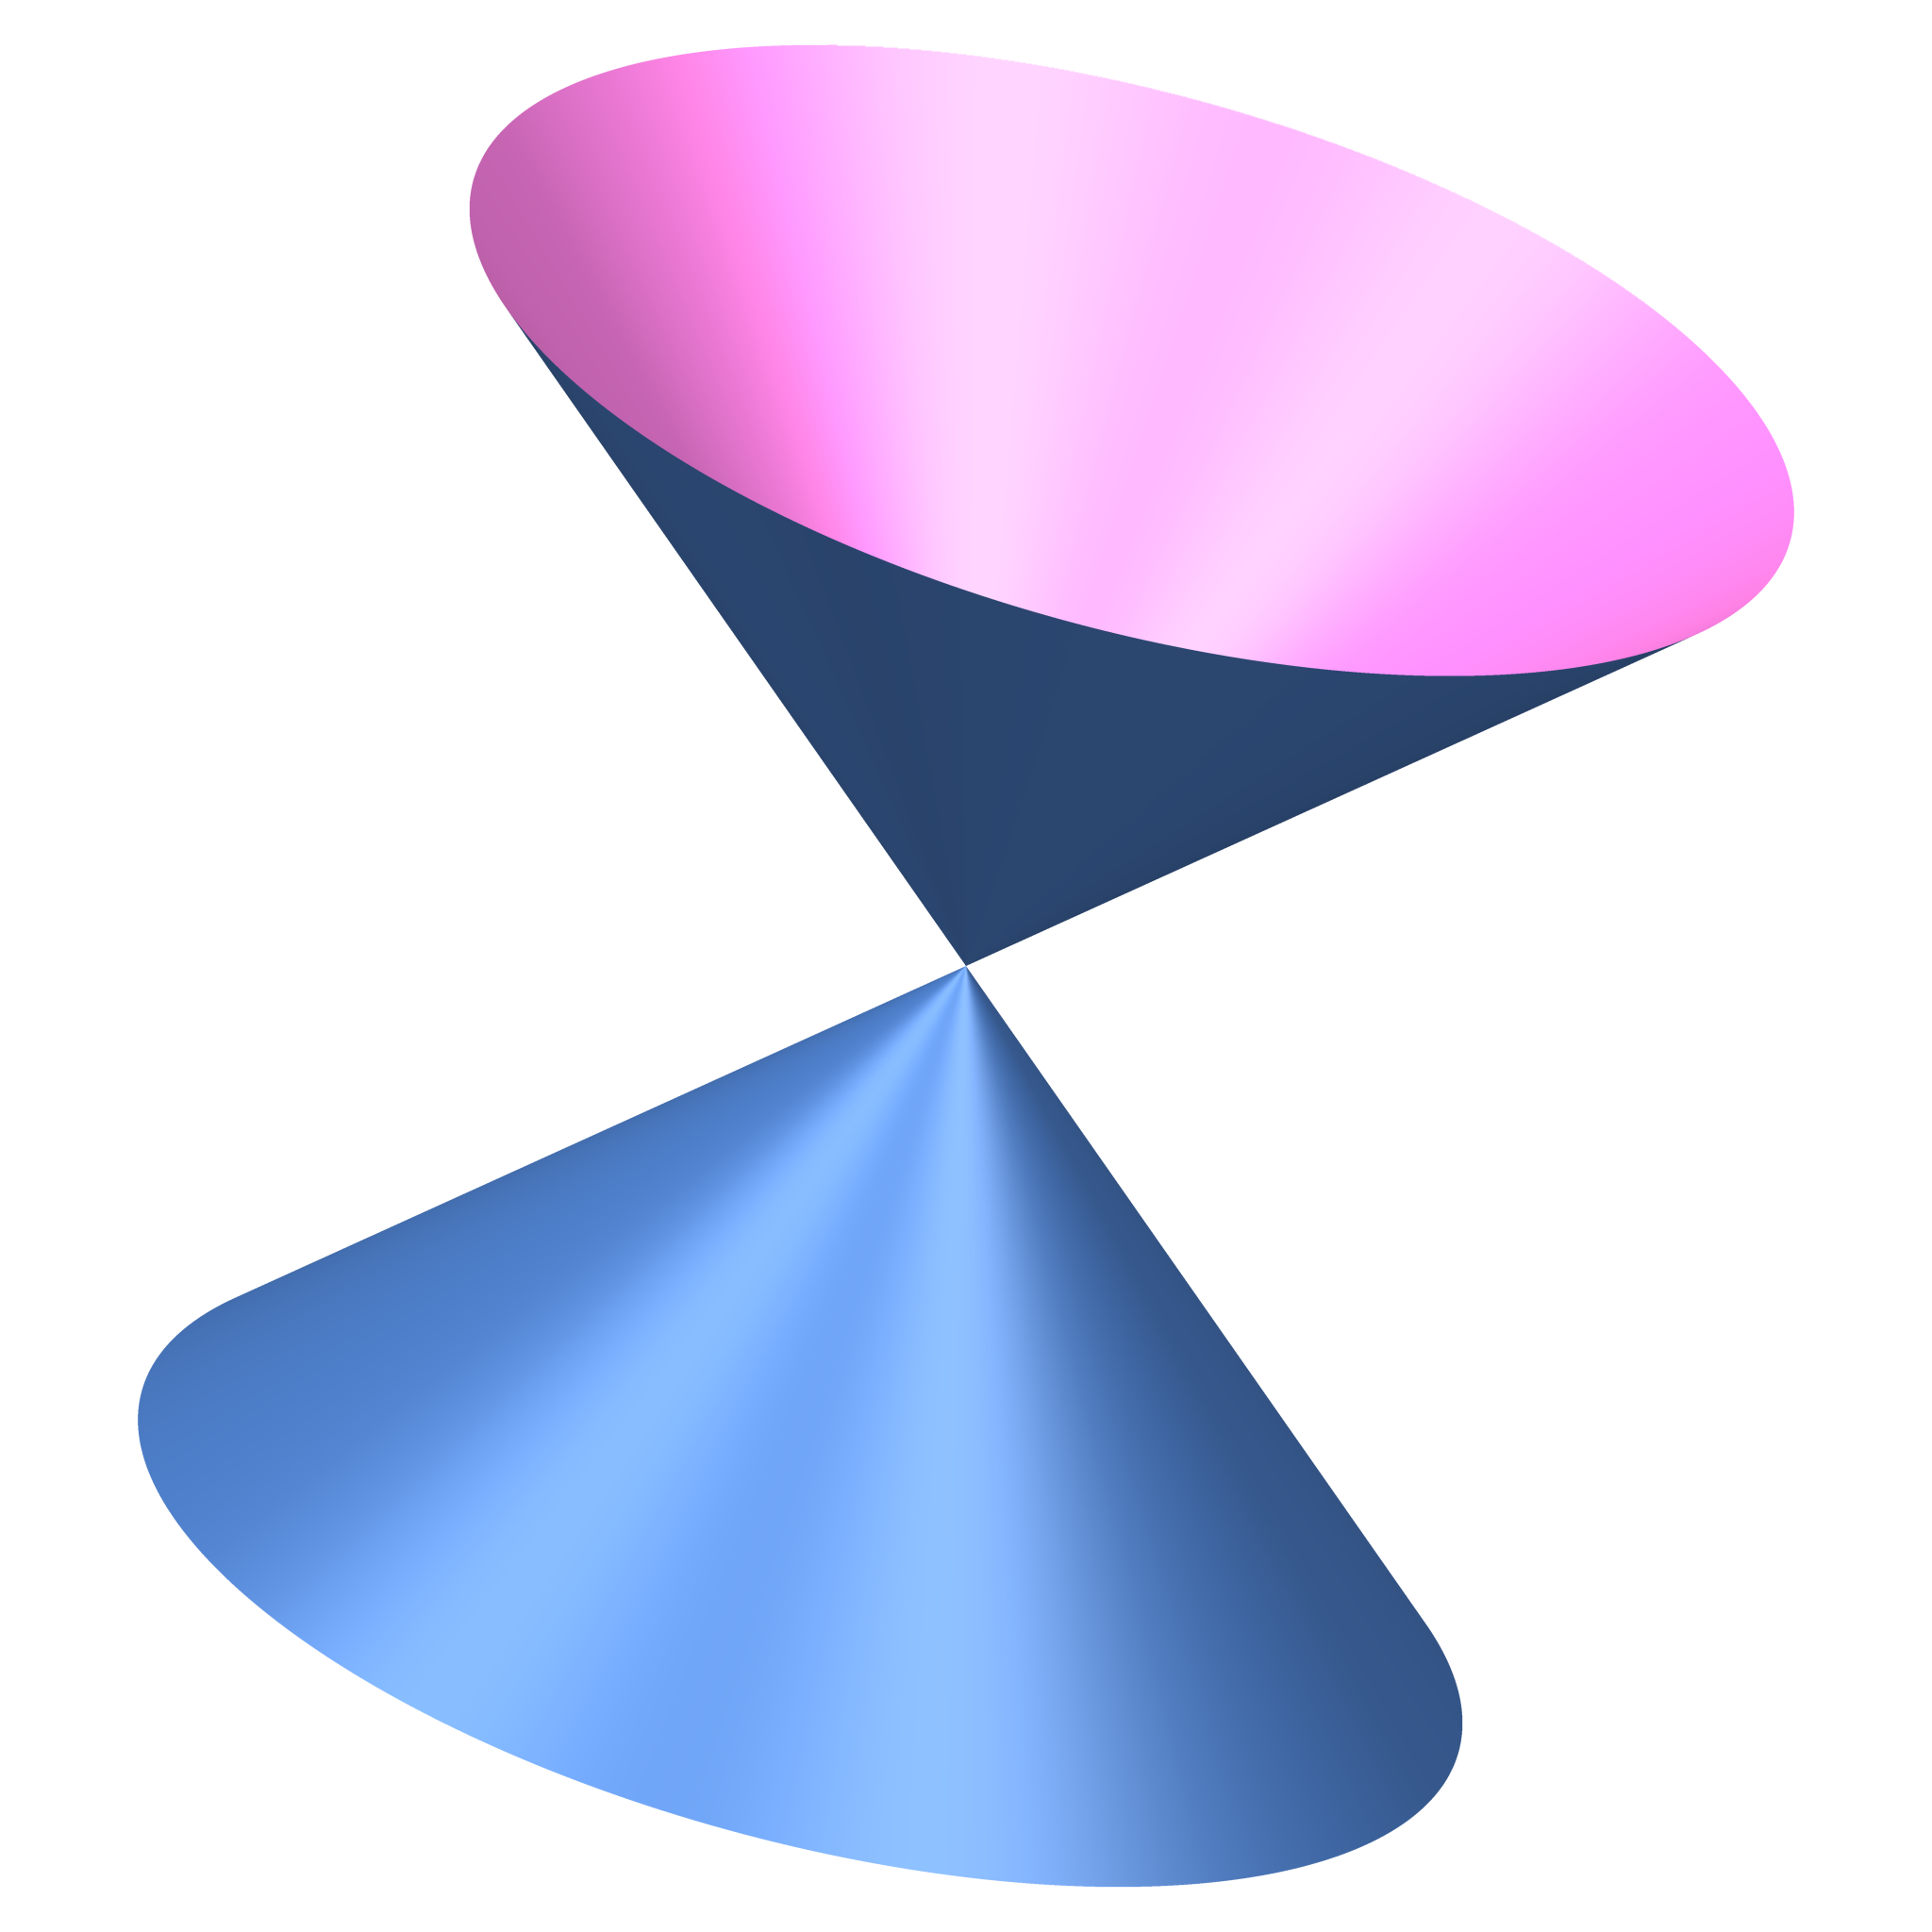
\includegraphics[width=0.3\linewidth]{../pictures/double_cone.png}
            \caption{The equation $h(x, y, z) = x^2 + y^2 - z^2 = 0$ gives rise
            to a double-cone shaped algebraic surface.}
            \label{fig:../pictures/double_cone}
        \end{figure}
        This surface has degree $d = 2$, and since all the terms have the same
        degree the defining polynomial is homogenous, and hence the surface is
        invariant under scaling.  
    \end{exmpl} 
    
    While there is a lot of fun to be had with algebraic surfaces of degree $2$
    there is a limit as to how exciting they are. Things get much more fun when
    we look at surfaces of higher degree. Consider for example the following
    surface of degree $3$.

    \begin{exmpl}[The ding-dong cubic]
        Let $h(x, y, z) = x^2 + y^2 - (1 - z)z^2$. Then the equation $h(x, y,
        z) = 0$ defines a surface of degree $d = 3$ (attributed to the
        $(1-z)z^2$ term). 
        \begin{figure}[h!]
            \centering
            
\includegraphics[width=0.3\linewidth]{../pictures/ding_dong.png}
            \caption{The ding-dong cubic given by the equation $h(x, y, z) =
            x^2 + y^2 - (1-z)z^2 = 0$.}
            \label{fig:../pictures/ding_dong}
        \end{figure}
        This surface also exhibits a singularity at the point $(0, 0, 0)$ where
        it passes through itself.
    \end{exmpl}
    
    Another very interesting  
\clearpage
\printbibliography
\end{document}
